\subsection{C++ e Java}

\begin{frame}{C++ e Java}
\framesubtitle{C++ e Java}
\begin{itemize}
    \item Linguagens muito relevantes atualmente muito importantes ao longo da história e no contexto atual de programação
    \item Orientação a objetos como um dos principais fatores de popularidade.

\end{itemize} 
\end{frame}

\begin{frame}{C++ e Java}
\framesubtitle{Popularidade}
    \begin{figure}
    	\centering
    	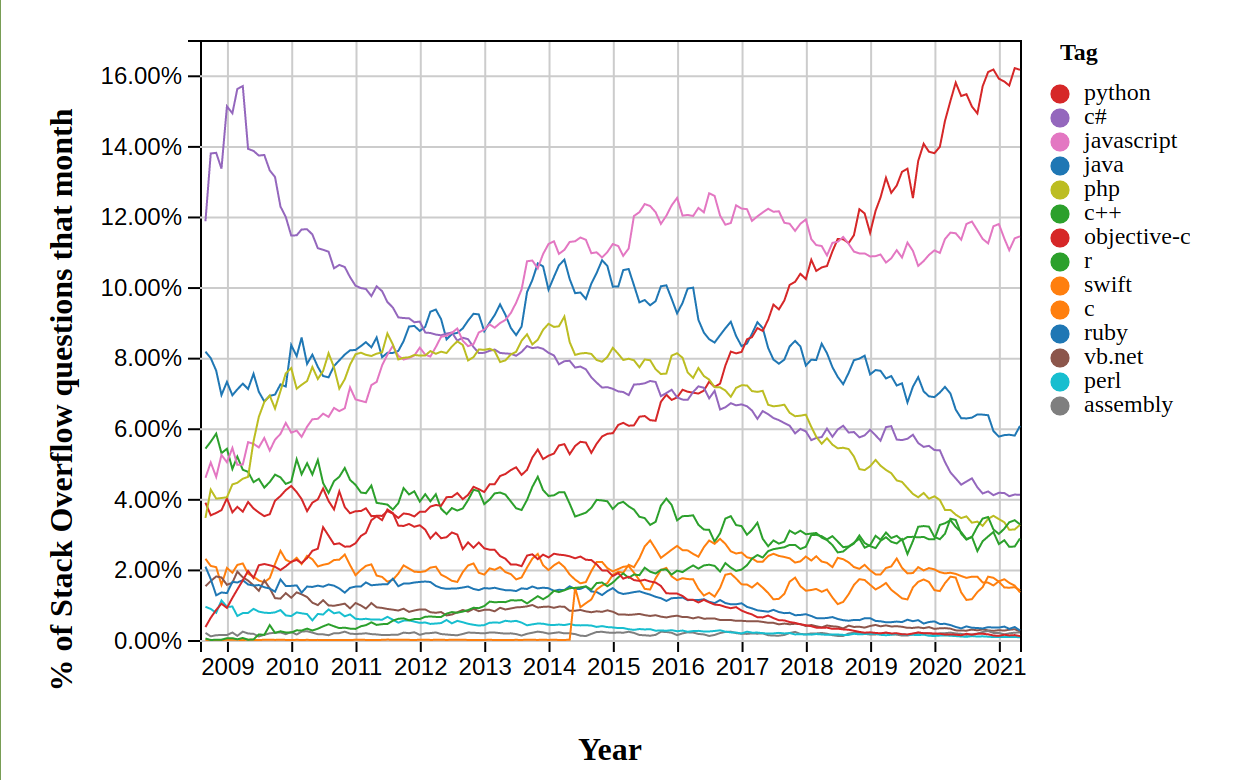
\includegraphics[width=0.9\linewidth]{img/image_pop.png}
    	\caption{Popularidade das linguagens de programação.\cite{stackoverflow}}
    	\label{fig:popularidade}
    \end{figure}
\end{frame}



\begin{frame}{C++ e Java}
\framesubtitle{C++}
\begin{itemize}
    \item Lançada por Bjarne Stroustrup em 1985.
    \item Planejada para ser um "C com classes".
    \item Adotou recursos de diversos paradigmas.
    \item Muito utilizada para contextos com recursos limitados ou que exijam alto desempenho, como software de sistema, embarcados, computação científica, gráficos, jogos,  etc.
\end{itemize} 
\end{frame}


\begin{frame}{C++ e Java}
\framesubtitle{Java}
\begin{itemize}
    \item Lançada pela Sun Microsystems em 1996.
    \item Fortemente orientada a objetos.
    \item Write Once, Run Anywhere (JVM).
    \item Uma das linguagens mais utilizadas atualmente no contexto de finanças, projetos corporativos, desenvolvimento de apps, etc.
\end{itemize} 
\end{frame}


\begin{frame}{C++ e Java}
\framesubtitle{Diferenças }
\begin{itemize}
    \item Ao contrário do C++, Java não suporta sobrecarga de operador ou herança múltipla para classes, embora herança múltipla seja compatível com interfaces.
    \item Gerenciamento de memória: Manual vs Garbage Colector.\cite{OOManagement}
    \item Passagem de argumentos por ponteiros vs por valor.

\end{itemize} 
\end{frame}

